\documentclass[11pt,twoside]{article}
\usepackage[utf8]{inputenc}
\usepackage[T1]{fontenc}
\usepackage[english,frenchb,spanish]{babel}
\usepackage{ifthen}
\def\localedef#1#2{
\ifthenelse{ \equal{\locale}{#1} }{
\selectlanguage{#2}
\expandafter\def\csname#1\endcsname ##1{##1}
 }{
\expandafter\def\csname#1\endcsname ##1{}
  }
}
\providecommand\locale{es}
\usepackage[margin=1in]{geometry}
\usepackage{fancyhdr}
\usepackage{amsfonts, amsmath, amssymb}
\usepackage[none]{hyphenat}
\usepackage{dsfont}
\usepackage{multirow}
\usepackage{graphicx}
\graphicspath{ {C:\Users\lm_lu\OneDrive\Documentos\GitHub\PrograMate201603126\Practica}}
\pagestyle{fancy}
\fancyhf{}
\fancyfoot{}
\cfoot{\thepage}
\lhead{MackTeck}
\rhead{\today}
\begin{document}
\begin{center}
\textbf{{\LARGE Datos Consultados}}\
\end{center}
\section*{Información:}
El siguiente es un documento con la información a la que usted accedió
\\
Nombre $ de $ usuario: $ Jmack$
\\Correo: $ jmackalvizures@hotmail.com$
\\A continuación se presenta una lista de los estados y las estaciones consultadas con su respectiva hora
\\
\begin{center}
\begin{tabular}{| c| c | c| c|c|}
\hline
Estados & Estaciones & Hora & Veces Consultadas\\ 
\hline\hline
\multirow{4}{10em}\\
KY & ANCHORAGE &  19:47 & 1\\
\hline
LA & ALEXANDRIA 5 SSE &  19:48 & 1\\
\hline
HI & AIEA FIELD 68 756 &  19:48 & 1\\
\hline
\end{tabular}\section*{Gráfica}
A continuación se presenta una gráfica con lo que consultó
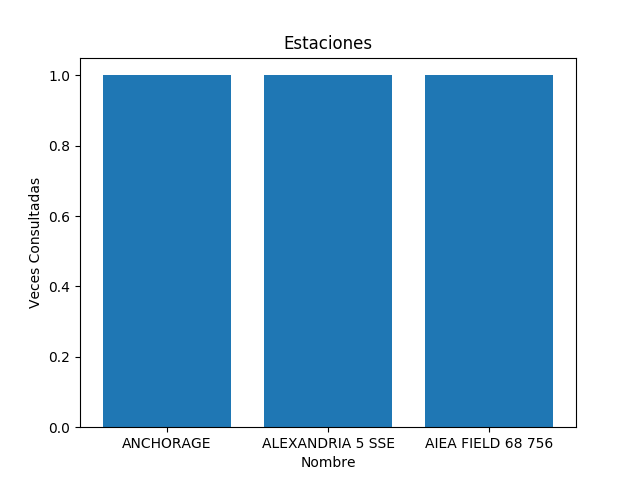
\includegraphics{grafica.png}

\end{center}
\end{document}